\def\mySecNum{18.2}
\mySection{\mySecNum~The lognormal distribution}
%-------------- start slide -------------------------------%{{{ 1 Def.
\begin{frame}[fragile,t]
\begin{mydefinition}
	A	random variable $Y$ is \textcolor{magenta}{\it lognormally distributed} with parameters $\mu$
	and  $\sigma>0$ if $\ln(Y)\sim N(\mu,\sigma^2)$.
\end{mydefinition}
\pause
\begin{mythm}
	The probability density function of $Y$	is given by
	\begin{align*}
		f_Y(y) = \frac{1}{y \sqrt{2\pi} \sigma} \exp\left(- \left(\frac{\ln(y)-\mu}{\sigma}\right)^2\right).
	\end{align*}
\end{mythm}
\pause
\begin{myproof}
	For $y>0$,
	\begin{align*}
		\bbP(Y\le y) & = \bbP\left(\ln(Y)\le \ln(y)\right)                                       \\
                 & = \bbP\left(\frac{\ln(Y)-\mu}{\sigma}\le \frac{\ln(y)-\mu}{\sigma}\right) \\
                 & = \Phi\left(\frac{\ln(y)-\mu}{\sigma}\right).
	\end{align*}
	\pause
	Hence,
	\begin{align*}
		f_Y(y) & = \frac{d}{d y}\Phi\left(\frac{\ln(y)-\mu}{\sigma}\right)                                                               \\
           & = \frac{1}{\sqrt{2\pi}} e^{-\frac{1}{2}\left(\frac{\ln(y)-\mu}{\sigma}\right)^2} \frac{d}{d y}\frac{\ln(y)-\mu}{\sigma} \\
           & = \frac{1}{y \sigma \sqrt{2\pi}} e^{-\frac{1}{2} \left(\frac{\ln(y)-\mu}{\sigma}\right)^2}.
	\end{align*}
	\myEnd
\end{myproof}
\end{frame}
%-------------- end slide -------------------------------%}}}
%-------------- start slide -------------------------------%{{{ 1 Plot pdf
\begin{frame}[fragile]
	\begin{minipage}{0.45\textwidth}
	\centering
	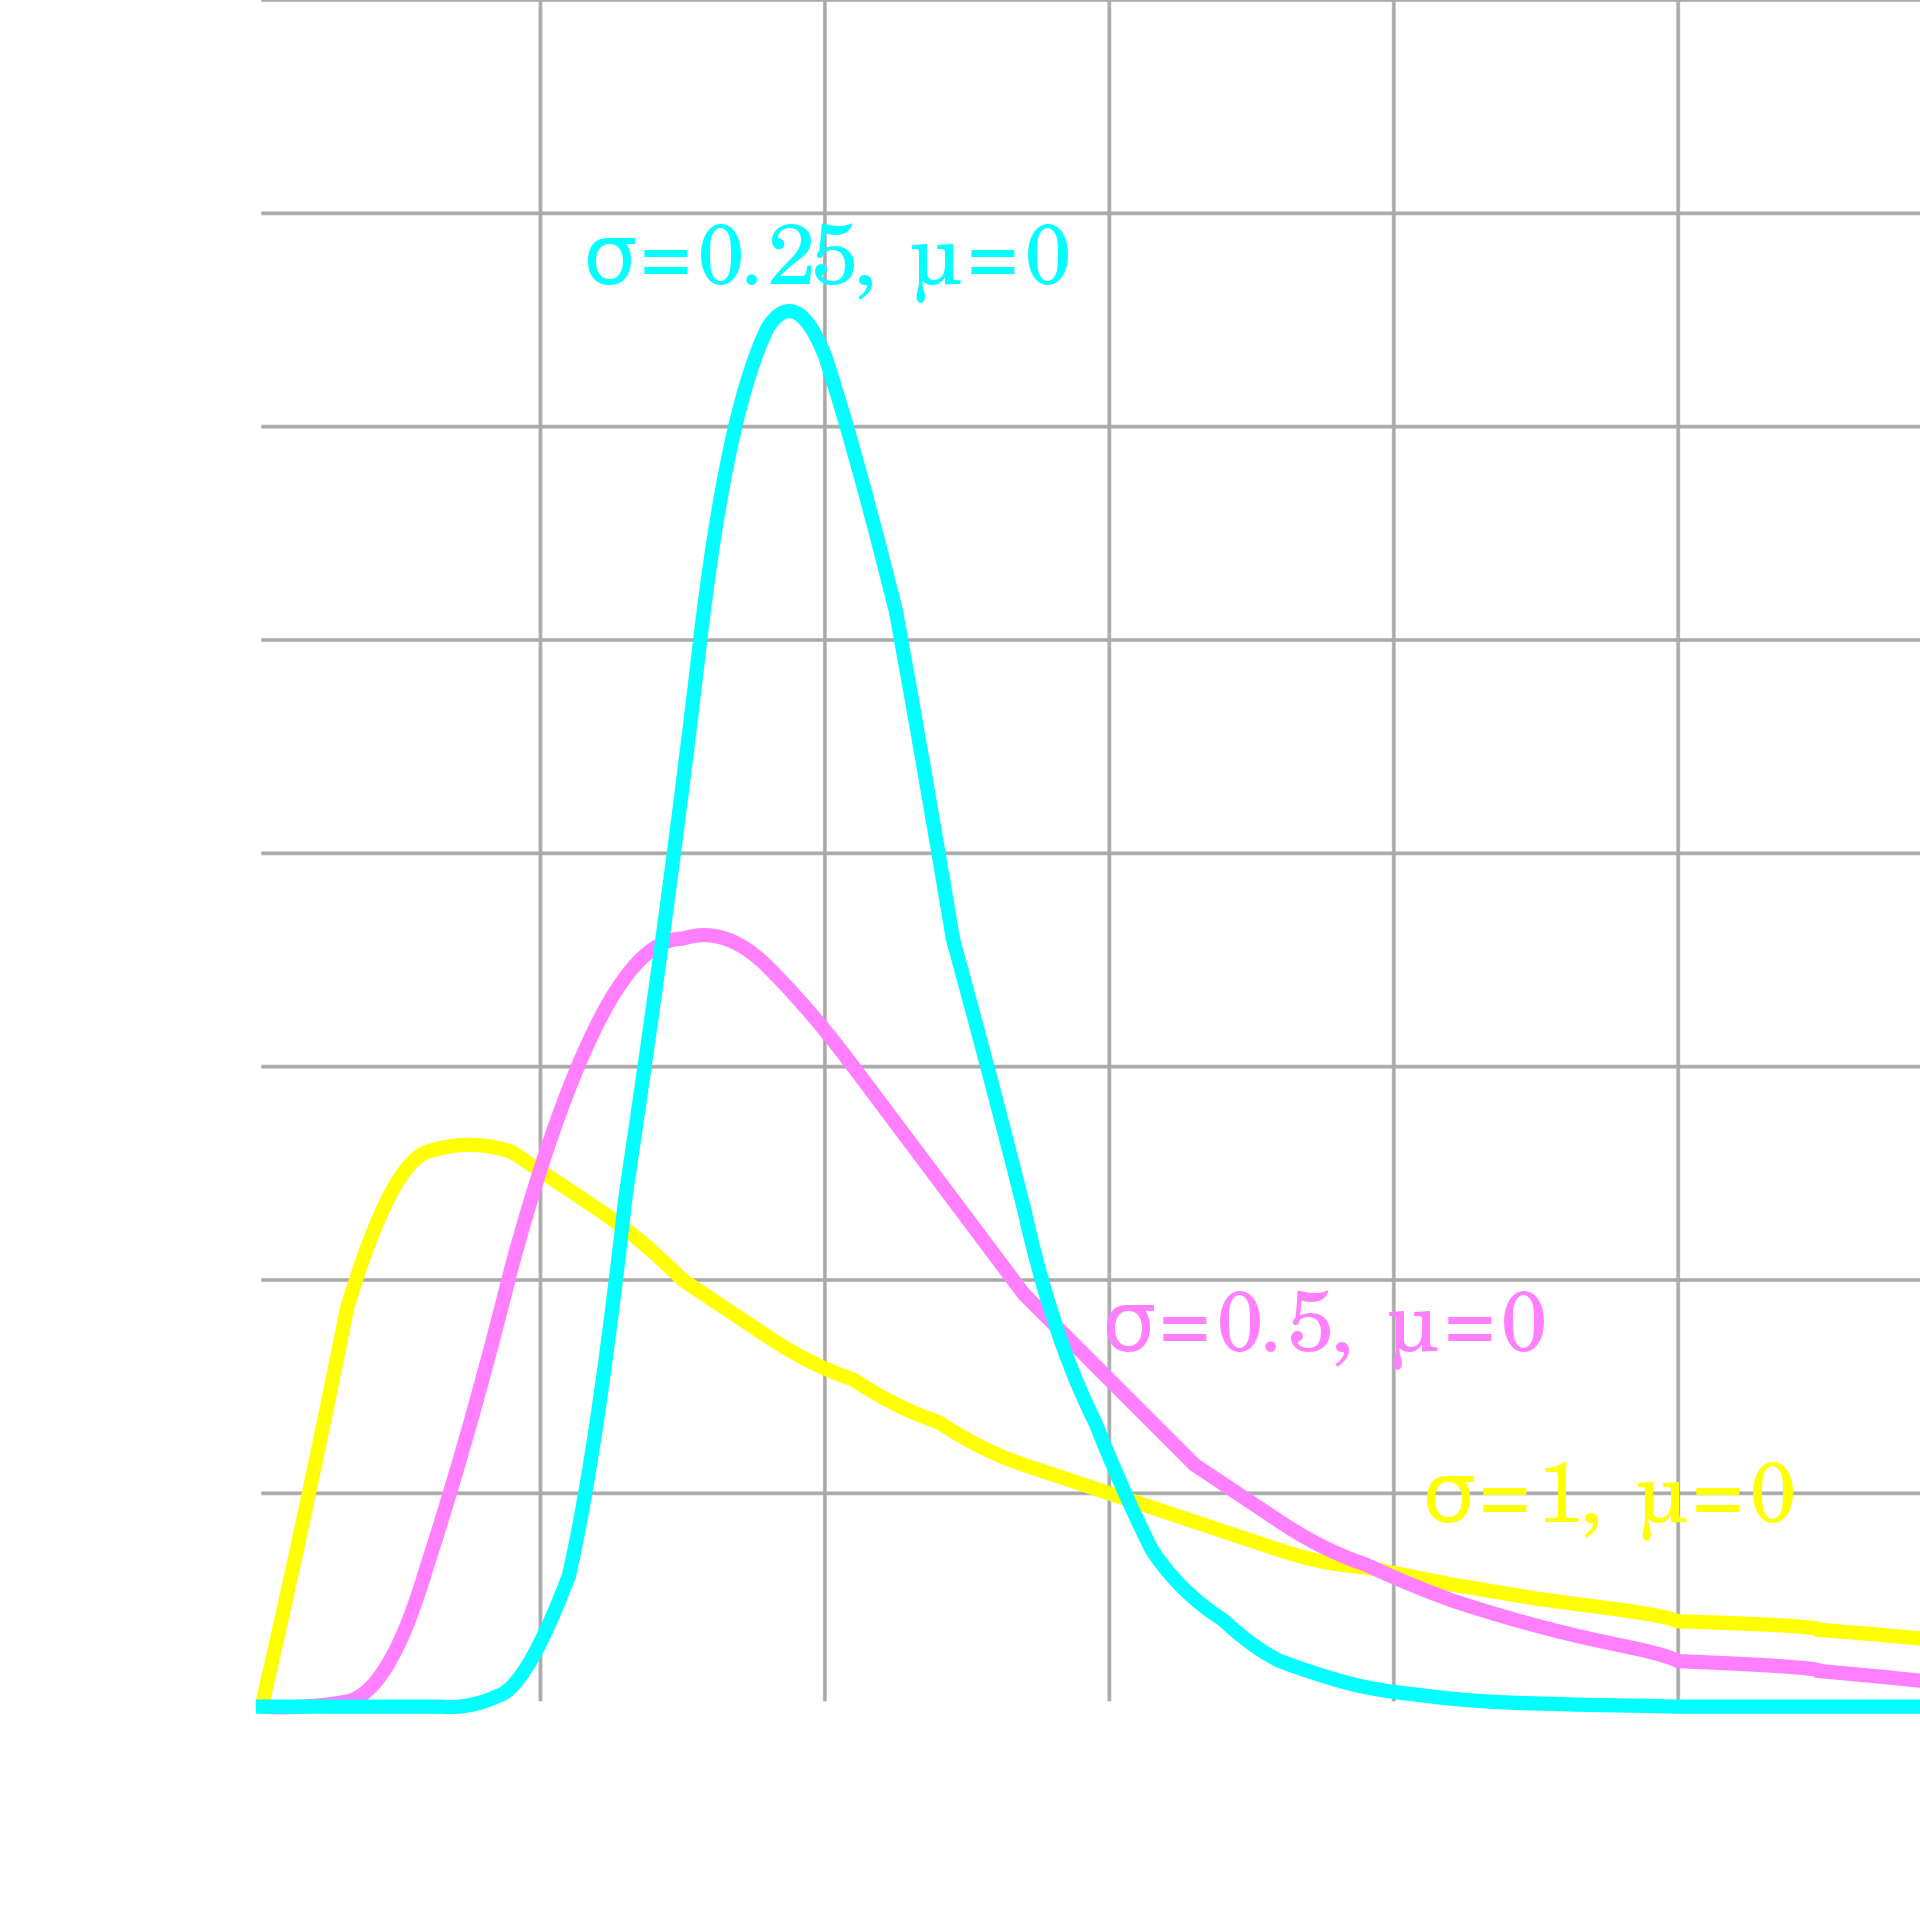
\includegraphics[scale=0.06]{figs/PDF-log_normal-neg.png}
	\end{minipage}
	\begin{minipage}{0.45\textwidth}
	\centering
	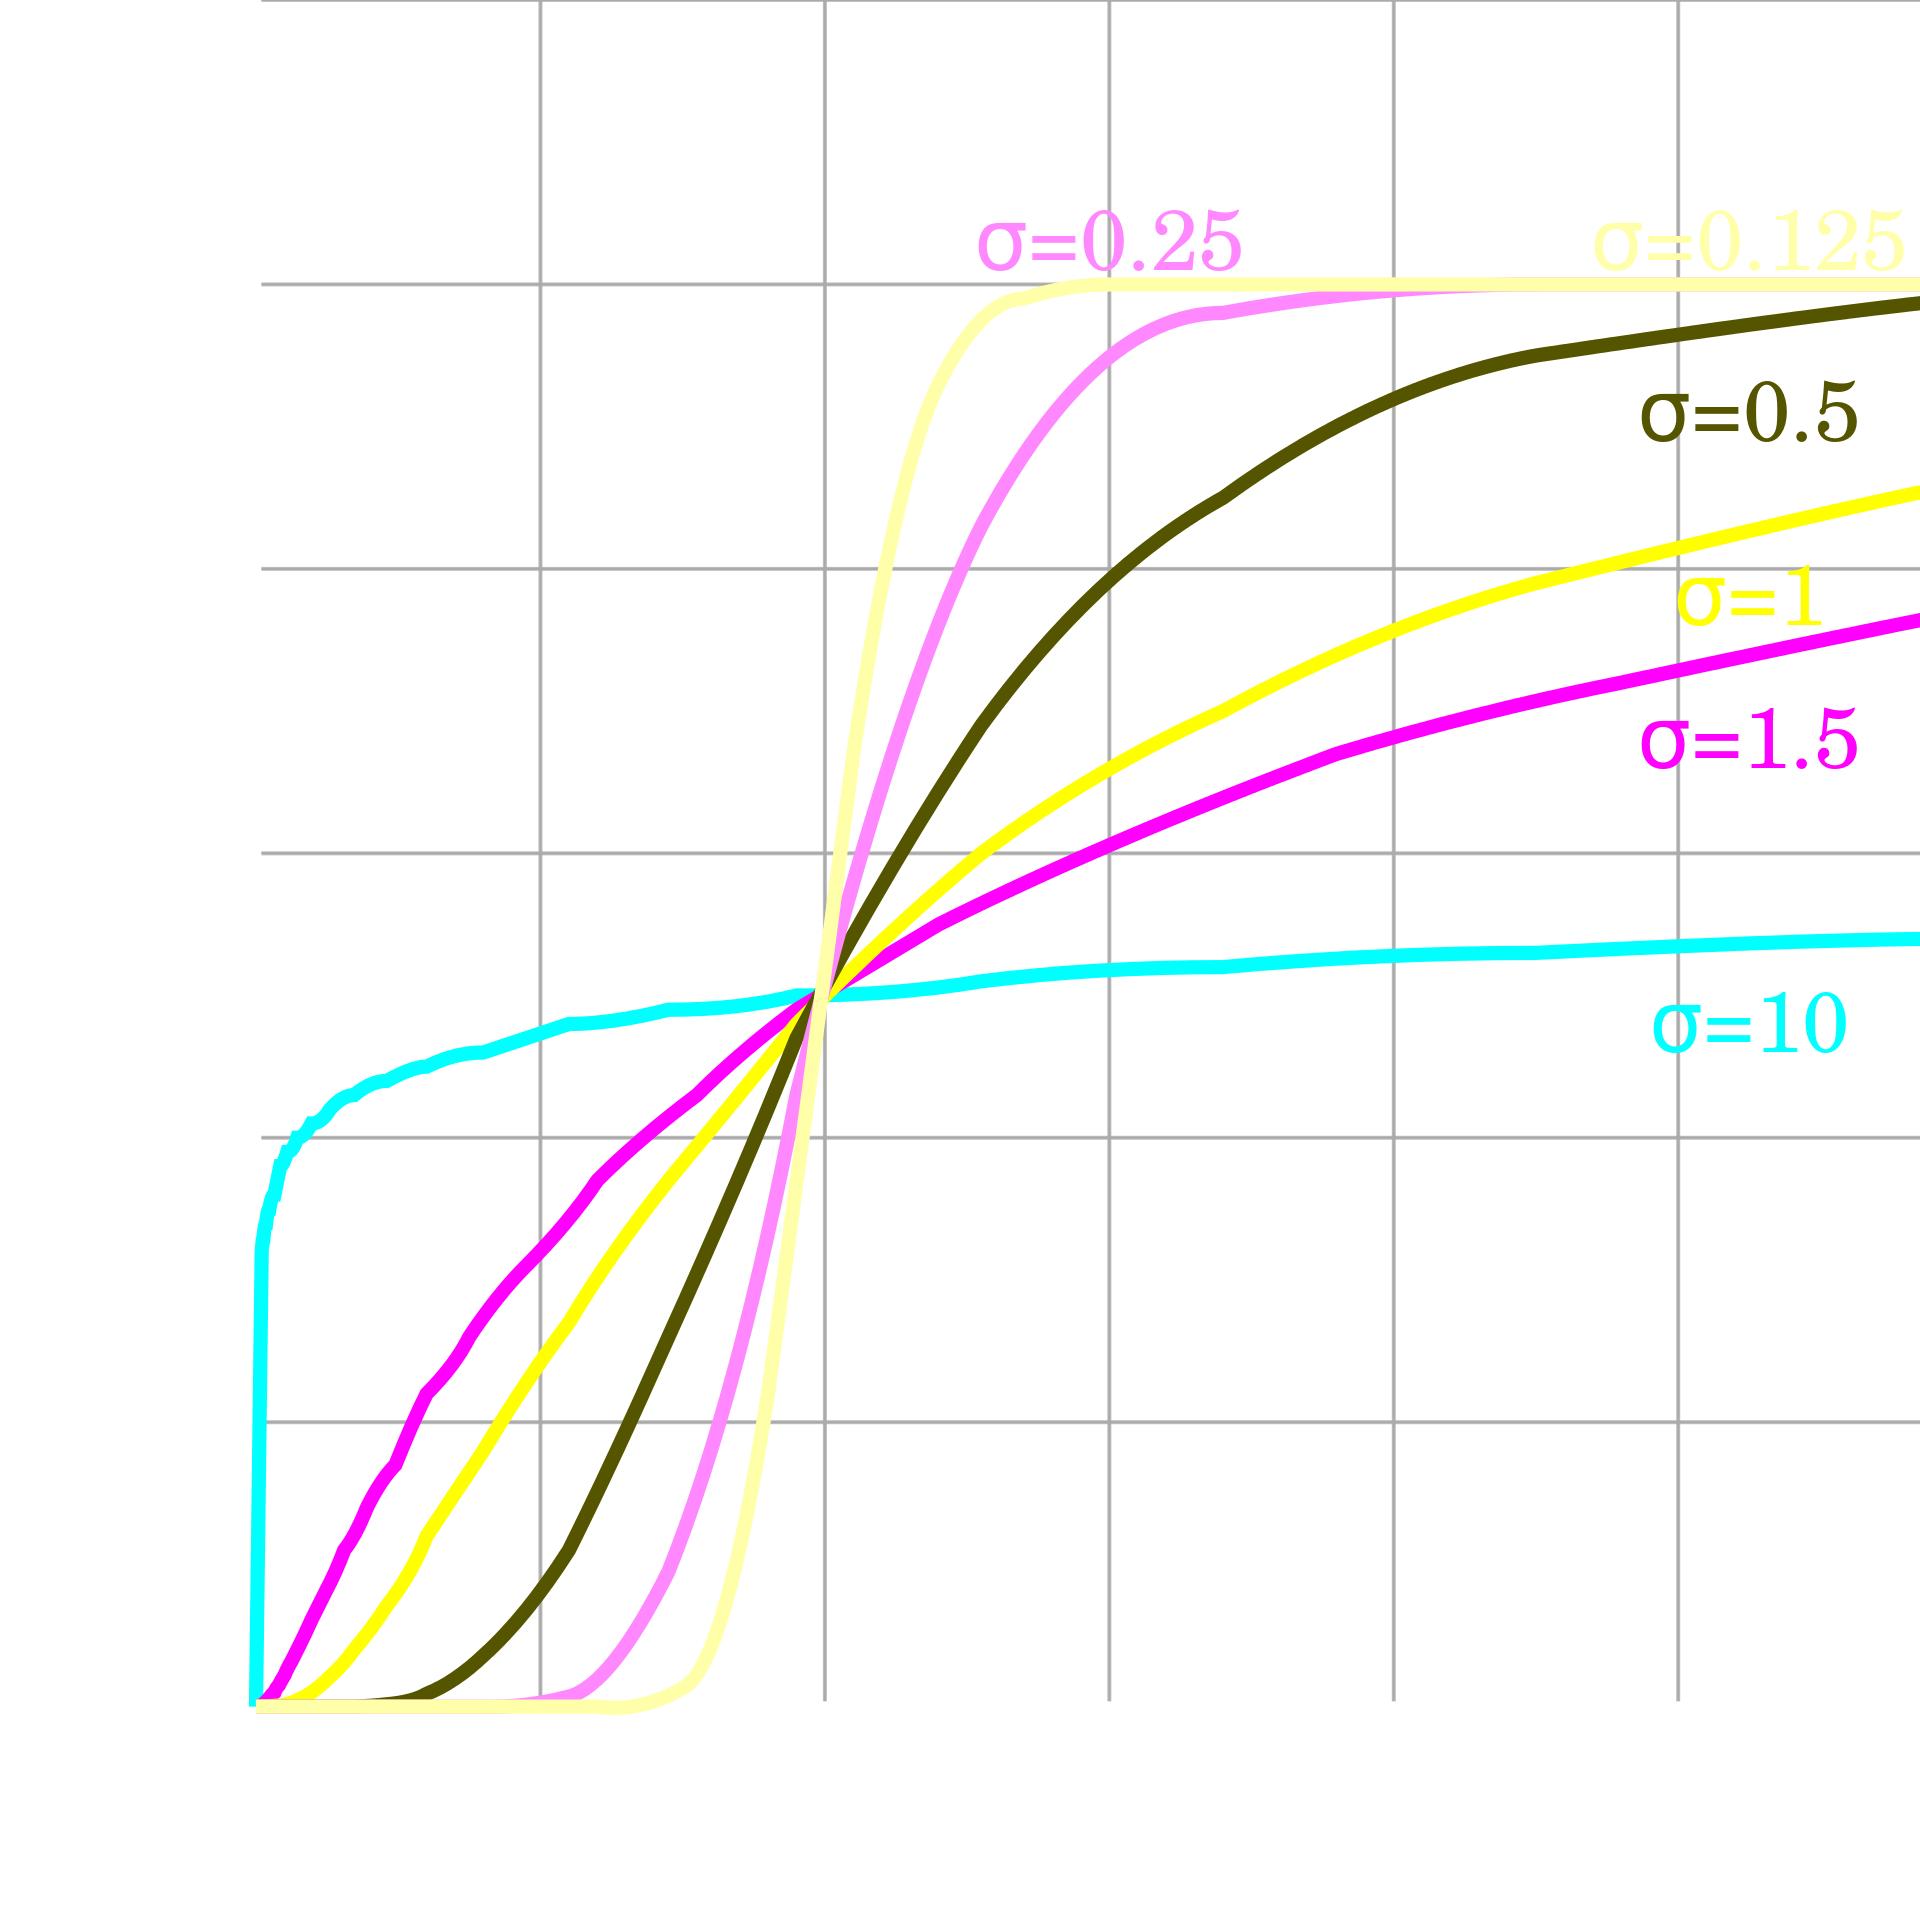
\includegraphics[scale=0.06]{figs/CDF-log_normal-neg.png}
\end{minipage}
\end{frame}
%-------------- end slide -------------------------------%}}}
%-------------- start slide -------------------------------%{{{ 1 Plot Change of variables
\begin{frame}[fragile,t]
\begin{center}
	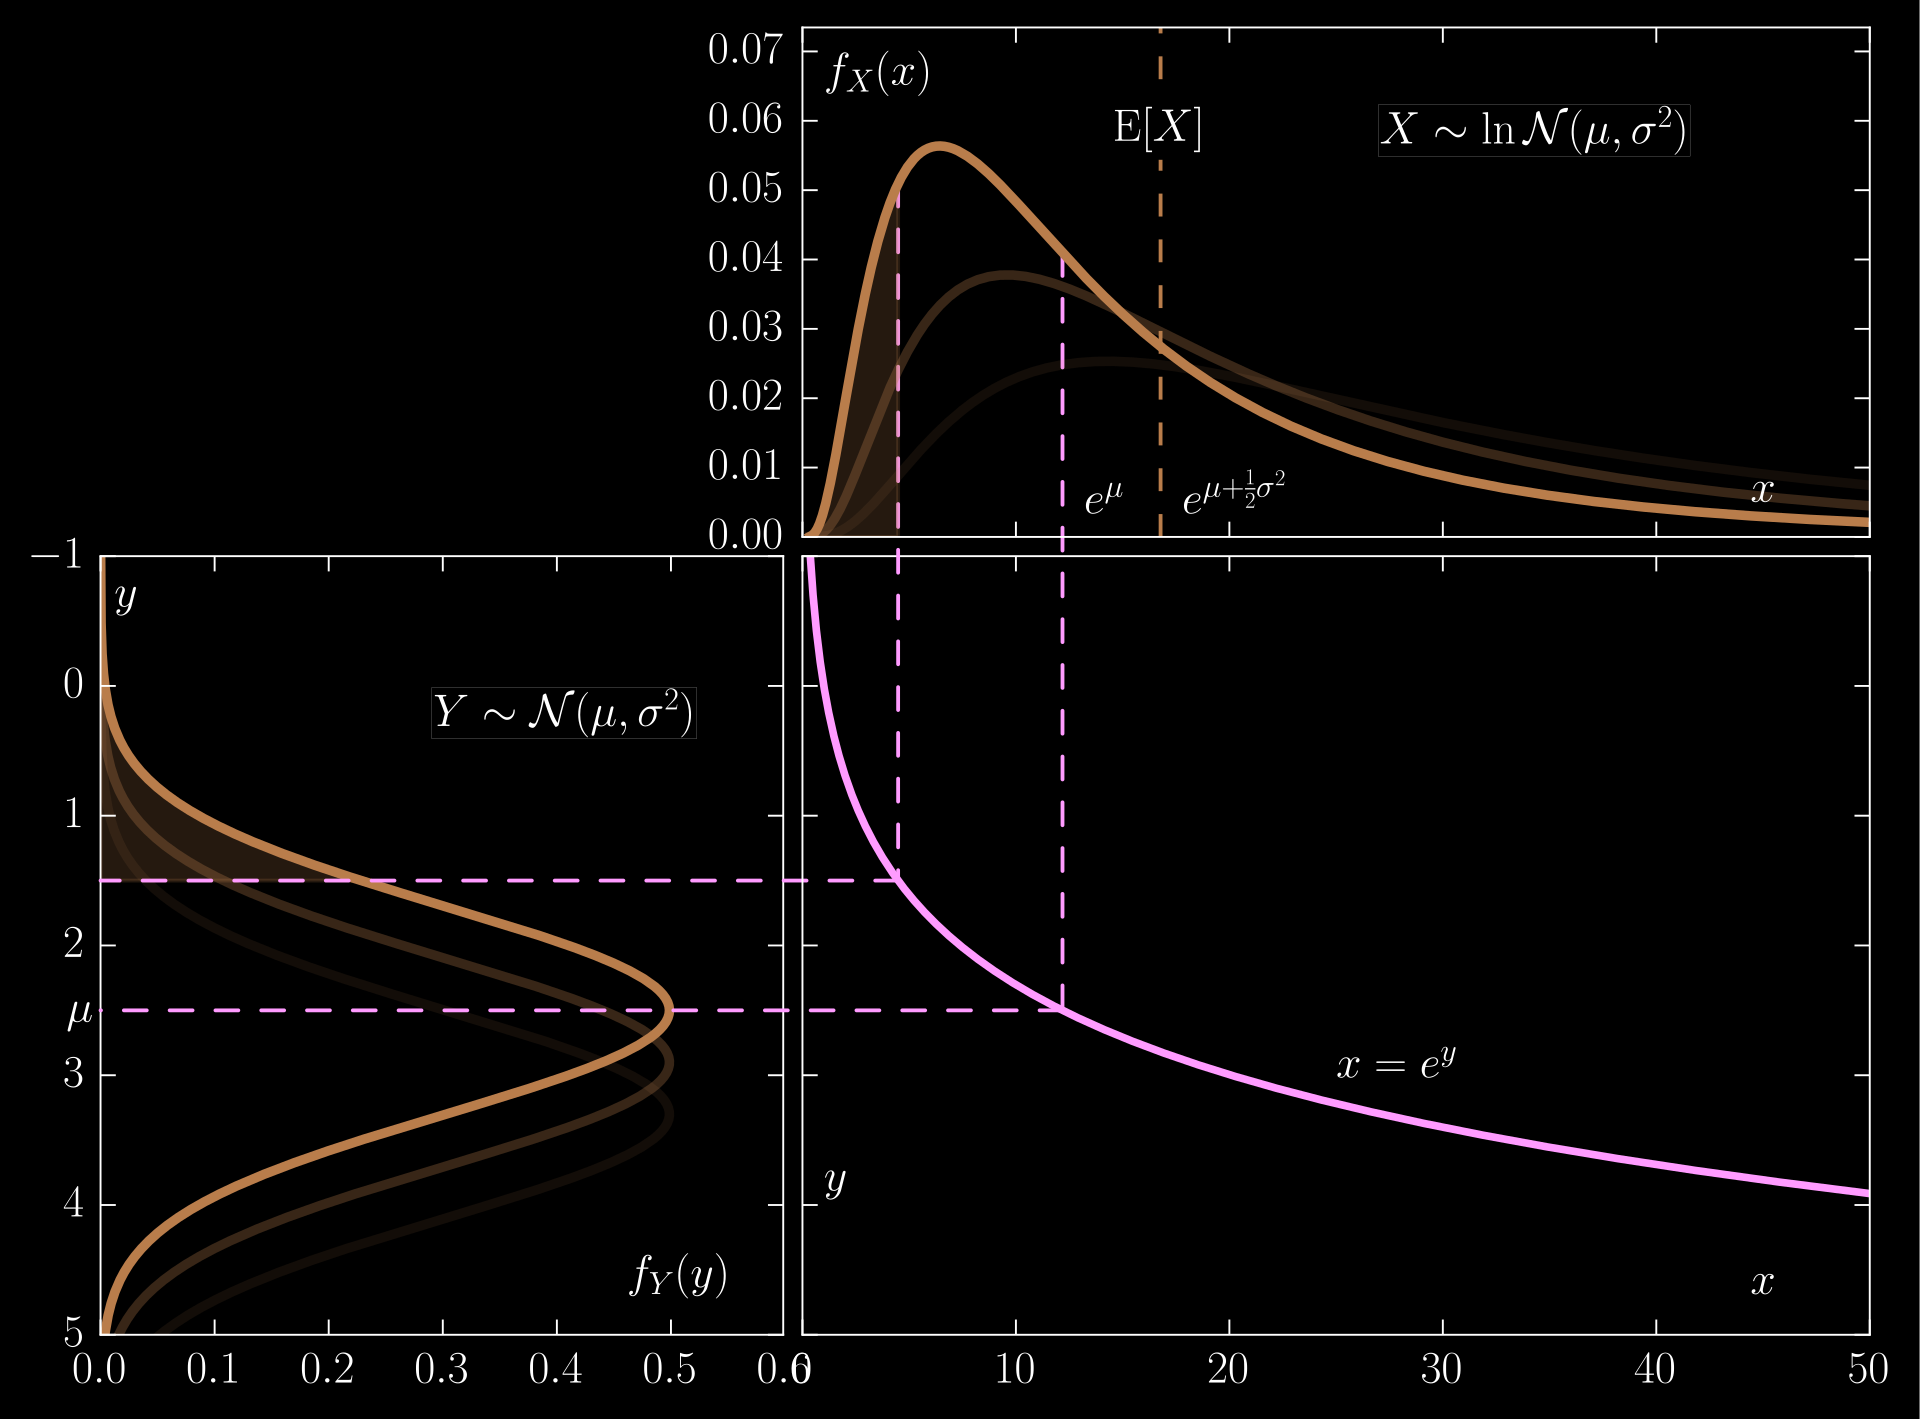
\includegraphics[scale=0.15]{figs/Lognormal_Distribution-neg.png}\footnote{Image from Wikipedia.}
\end{center}
\end{frame}
%-------------- end slide -------------------------------%}}}
%-------------- start slide -------------------------------%{{{ 1
\begin{frame}[fragile,t]
	\begin{mythm}
		If $Y_1$ and $Y_2$ are lognormally distributed, so is $Y_1Y_2$.
	\end{mythm}
	\bigskip
	\pause
	\begin{myproof}
		Since $Y_1$ and $Y_2$ are lognormally distributed, $\ln(Y_1)$ and $\ln(Y_2)$ are normally
		distributed. Hence,
		\begin{align*}
			\ln(Y_1) + \ln(Y_2) = \ln(Y_1Y_2)
		\end{align*}
		is normally distributed too. Therefore, $Y_1Y_2$ is lognormally distributed.
		\myEnd
	\end{myproof}
\end{frame}
%-------------- end slide -------------------------------%}}}
% -------------- start slide -------------------------------%{{{ 1
% \begin{frame}[fragile,t]
% \begin{mythm}
% 	If $\ln(Y)\sim N(\mu,\sigma^2)$, then the density of $Y$ is given by
% 	\begin{align*}
% 		f_Y(y) = \frac{1}{y \sigma \sqrt{2\pi}} e^{-\frac{1}{2} \left(\frac{\ln(y)-\mu}{\sigma}\right)^2}.
% 	\end{align*}
% \end{mythm}
% \bigskip
% \pause
% \begin{myproof}
% 	For $y>0$,
% 	\begin{align*}
% 		\bbP(Y\le y) & = \bbP\left(\ln(Y)\le \ln(y)\right)                                       \\
%                  & = \bbP\left(\frac{\ln(Y)-\mu}{\sigma}\le \frac{\ln(y)-\mu}{\sigma}\right) \\
%                  & = \Phi\left(\frac{\ln(y)-\mu}{\sigma}\right).
% 	\end{align*}
% 	\pause
% 	Hence,
% 	\begin{align*}
% 		f_Y(y) & = \frac{d}{d y}\Phi\left(\frac{\ln(y)-\mu}{\sigma}\right)                                                               \\
%            & = \frac{1}{\sqrt{2\pi}} e^{-\frac{1}{2}\left(\frac{\ln(y)-\mu}{\sigma}\right)^2} \frac{d}{d y}\frac{\ln(y)-\mu}{\sigma} \\
%            & = \frac{1}{y \sigma \sqrt{2\pi}} e^{-\frac{1}{2} \left(\frac{\ln(y)-\mu}{\sigma}\right)^2}.
% 	\end{align*}
% 	\myEnd
% \end{myproof}
% \end{frame}
% -------------- end slide -------------------------------%}}}
%-------------- start slide -------------------------------%{{{ 1
\begin{frame}[fragile,t]
	Recall that the moment generating function of the normal random variable $X\sim
	N(\mu,\sigma^2)$ is
	\begin{align}
		\label{E:MomentGen}
		\E\left(e^{t\: X}\right) = e^{\mu t+\sigma^2 t^2/2}, \qquad \text{for all $t\in\R$.}
	\end{align}
	\bigskip
	\begin{remark}
		If $Y$ is lognormally distributed with parameters $\mu$ and $\sigma$, then
		\begin{align*}
			\E\left(Y^t\right) =  e^{\mu t+\sigma^2 t^2/2}, \qquad \text{for all $t\in\R$.}
		\end{align*}
	\end{remark}
	\bigskip
	\begin{remark}
		By \textcolor{magenta}{\it Jensen's inequality}, if $g$ is a convex function, then
		\begin{align*}
			\E\left(g(X)\right) \le g\left(\E(X)\right).
		\end{align*}
		Hence, for $g(x)=e^x$, we see that
		\begin{align*}
			\E\left(e^X\right) \le e^{\E(X)}.
		\end{align*}
		This is consistent with our computations above because
		\begin{align*}
			LHS=e^{\mu+\sigma^2/2} \ge e^{\mu} = RHS.
		\end{align*}
	\end{remark}
\end{frame}
%-------------- end slide -------------------------------%}}}
%-------------- start slide -------------------------------%{{{ 1
\begin{frame}[fragile,t]
\begin{mythm}
	If $Y$ is lognormally distributed such that $\ln(Y)\sim N(\mu,\sigma^2)$, then
	\begin{align*}
		\E(Y) = e^{\mu + \frac{1}{2}\sigma^2} \quad \text{and} \quad
		\Var(Y) = e^{2\mu+\sigma^2}\left(e^{\sigma^2}-1\right).
	\end{align*}
\end{mythm}
\bigskip
\pause
\begin{myproof}
	Let $X=\ln(Y)$. By \eqref{E:MomentGen},
	\begin{align*}
		\E\left(Y\right) = \E\left(e^X\right) = e^{\mu + \frac{1}{2}\sigma^2}
	\end{align*}
	and
	\begin{align*}
		\E(Y^2) = \E\left(e^{2X}\right) = e^{2\mu + 2 \sigma^2}.
	\end{align*}
	Therefore,
	\begin{align*}
		\Var(Y) = \E(Y^2) - \E(Y)^2 = e^{2\mu + 2 \sigma^2} - e^{2\left(\mu +
		\frac{1}{2}\sigma^2\right)}= e^{2\mu+\sigma^2}\left(e^{\sigma^2}-1\right).
	\end{align*}
	\myEnd
\end{myproof}
\end{frame}
%-------------- end slide -------------------------------%}}}
